\begin{frame}
\frametitle{About This Work...}

\emph{A Foundation for Efficient Indoor Distance-Aware Query Processing}.~\cite{DBLP:conf/icde/LuYCJ11} \\
H.~Lu, X.~Cao, and C.~S. Jensen.\\~\\

\begin{itemize}
  \item Published at \emph{ICDE' 2012}.
  \item First time to propose a distance-aware indoor space model that integrates indoor distance seamlessly.
  \item Accompanying, efficient algorithms for computing indoor distances.
  \item Indexing framework that accommodates indoor distances.
\end{itemize}

\end{frame}

%------------------------------------------------

\begin{frame}
\frametitle{Motivation}

\begin{itemize}
  \item A variety of LBS services are useful in indoor space.
    \begin{fitemize}
      \item a museum guidance service in a complex exhibition
      \item boarding reminder service in an airport, to remind the passengers especially those far away from their gates or departures
    \end{fitemize}

  \item Such indoor LBSs will benefit from the availability of accurate indoor distances.
    \begin{fitemize}
      \item indoor space entities enable as well as constrain indoor movement, thus makes traditional space model for Euclidean/spatial network spaces unsuitable.
      \item existing indoor space models~\cite{becker2005location, li2008lattice, becker2009multilayered} pay little attention to indoor distances.
    \end{fitemize}

\end{itemize}

\end{frame}

%------------------------------------------------

\begin{frame}
\frametitle{Indoor Topology Mapping Structures}

Mapping $D2P$ maps a door $d_k$ to one or two partition pairs~\footnote{\ssize{the basic assumption that a door corresponds to two doors can be extended by converting a door to multiple doors.}} $(v_i, v_j)$ such that one can move from partition~\footnote{\ssize{a partition indicates a room, a hallway or a staircase.}} $v_i$ to partition $v_j$ through door $d_k$:
\pause
\begin{equation}
 D2P: \mathcal{S}_{door} \rightarrow 2^{\mathcal{S}_{partition}} \times 2^{\mathcal{S}_{partition}}
\end{equation}
\pause
For \emph{enterable partition} of door $d_k$:
\pause
\begin{equation}
 D2P_{\sqsupset}: \mathcal{S}_{door} \rightarrow 2^{\mathcal{S}_{partition}}
\end{equation}
\pause
For \emph{leaveable partition} of door $d_k$:
\pause
\begin{equation}
 D2P_{\sqsubset}: \mathcal{S}_{door} \rightarrow 2^{\mathcal{S}_{partition}}
\end{equation}
\end{frame}

%------------------------------------------------

\begin{frame}
\frametitle{Indoor Topology Mapping Structures}


The mapping $P2D_{\sqsupset}$ maps a partition $v$ to all the doors through which one can enter $v$:
\pause
\begin{equation}
 P2D_{\sqsupset}: \mathcal{S}_{partition} \rightarrow 2^{\mathcal{S}_{door}}
\end{equation}
\pause
The mapping $P2D_{\sqsubset}$ maps a partition $v$ to all the doors through which one can leave $v$:
\pause
\begin{equation}
 P2D_{\sqsubset}: \mathcal{S}_{partition} \rightarrow 2^{\mathcal{S}_{door}}
\end{equation}
\pause
The mapping $P2D$ is used when there's no need to differentiate the directionality:
\pause
\begin{equation}
 P2D(v_i): P2D_{\sqsupset}(v_i) \cup P2D_{\sqsubset}(v_i)
\end{equation}
\end{frame}

%------------------------------------------------

\begin{frame}
\frametitle{Accessibility Base Graph}

\begin{columns}[c]

  \column{0.52\textwidth}
  \vspace{-15pt}
  \begin{figure}[tb]
    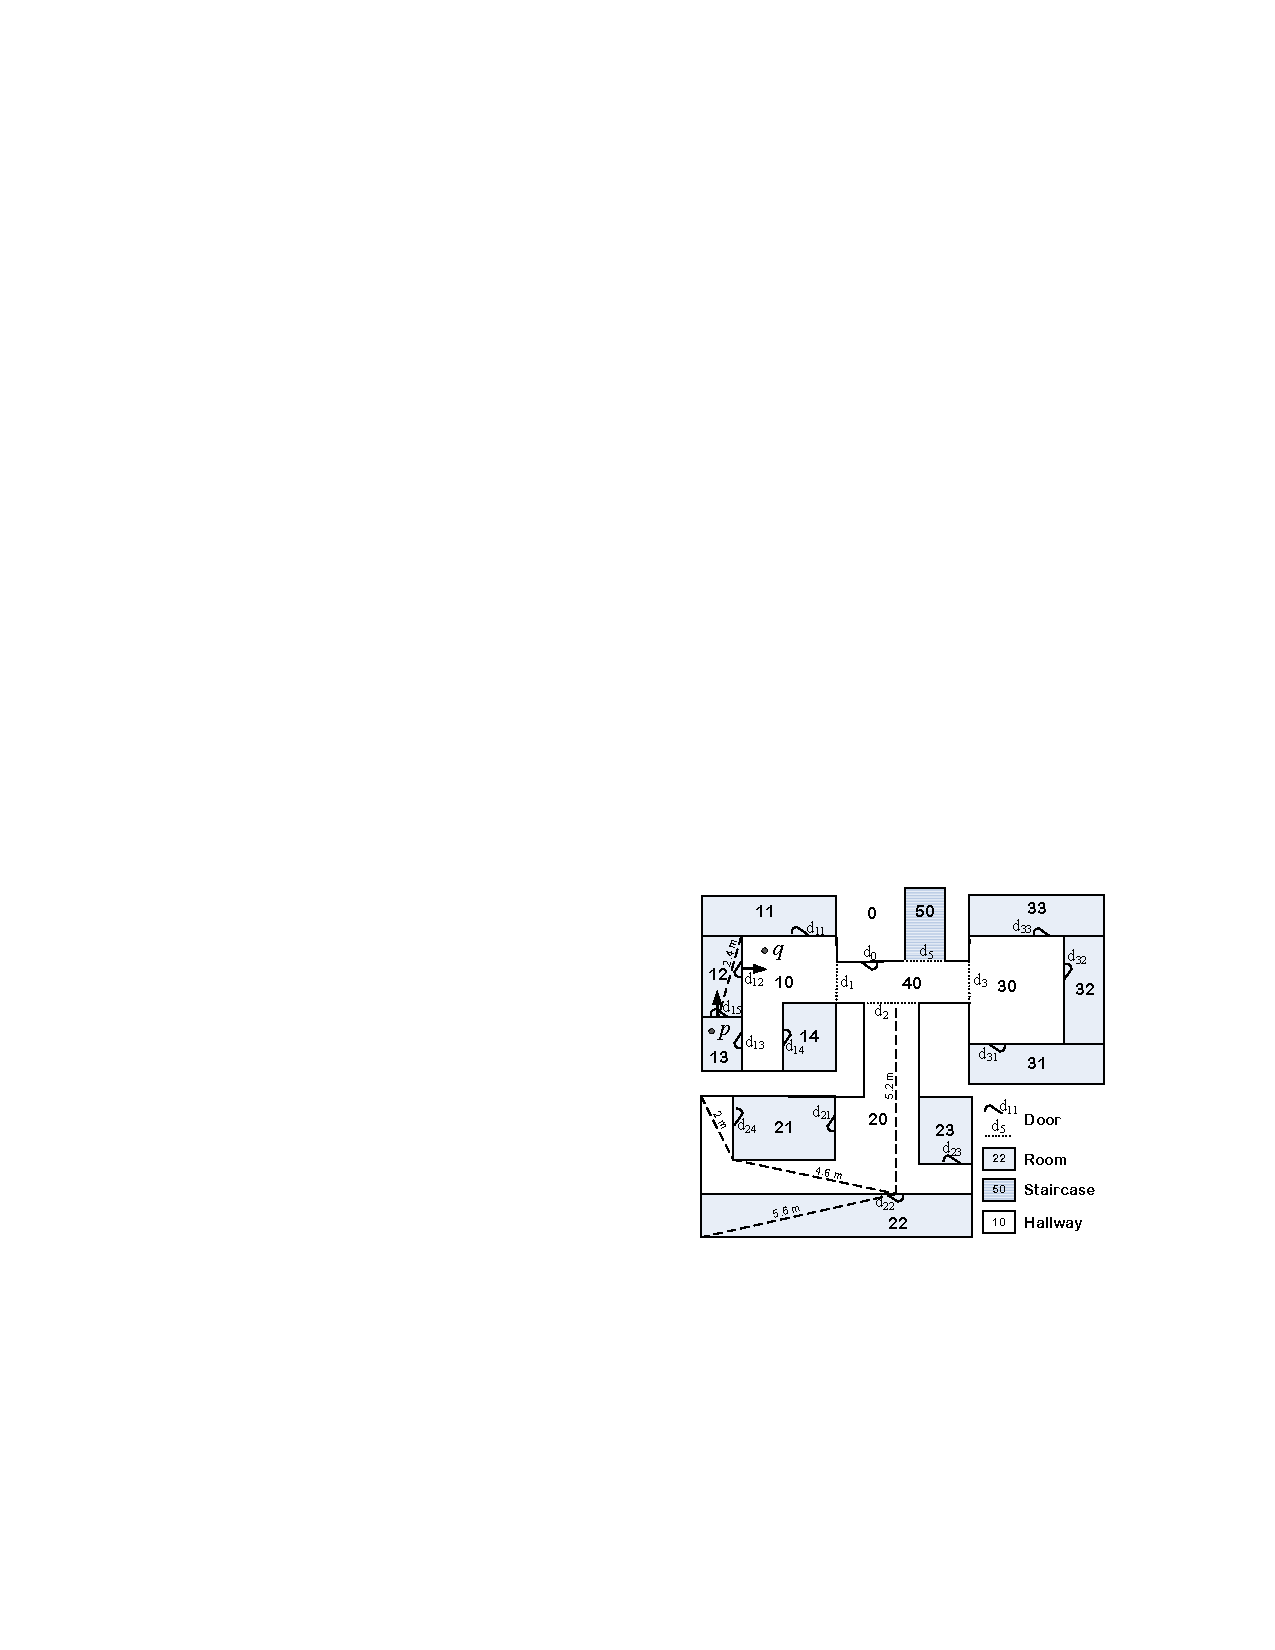
\includegraphics[width=0.85\columnwidth]{figures/2-5/2-5-1.pdf}
  \end{figure}
  \begin{example}
    \textrm{
    \ssize{
      $D2P_{\sqsupset}(d_{12}) = \{ v_{10}\}$, $D2P_{\sqsubset}(d_{12}) = \{ v_{12}\}$
      $P2D_{\sqsupset}(v_{13}) = \{ d_{13}\}$, $P2D_{\sqsubset}(v_{13}) = \{ d_{13}, d_{15}\}$
    }
    }
  \end{example}

  \column{0.48\textwidth}
  \vspace{-15pt}
  \begin{figure}[tb]
    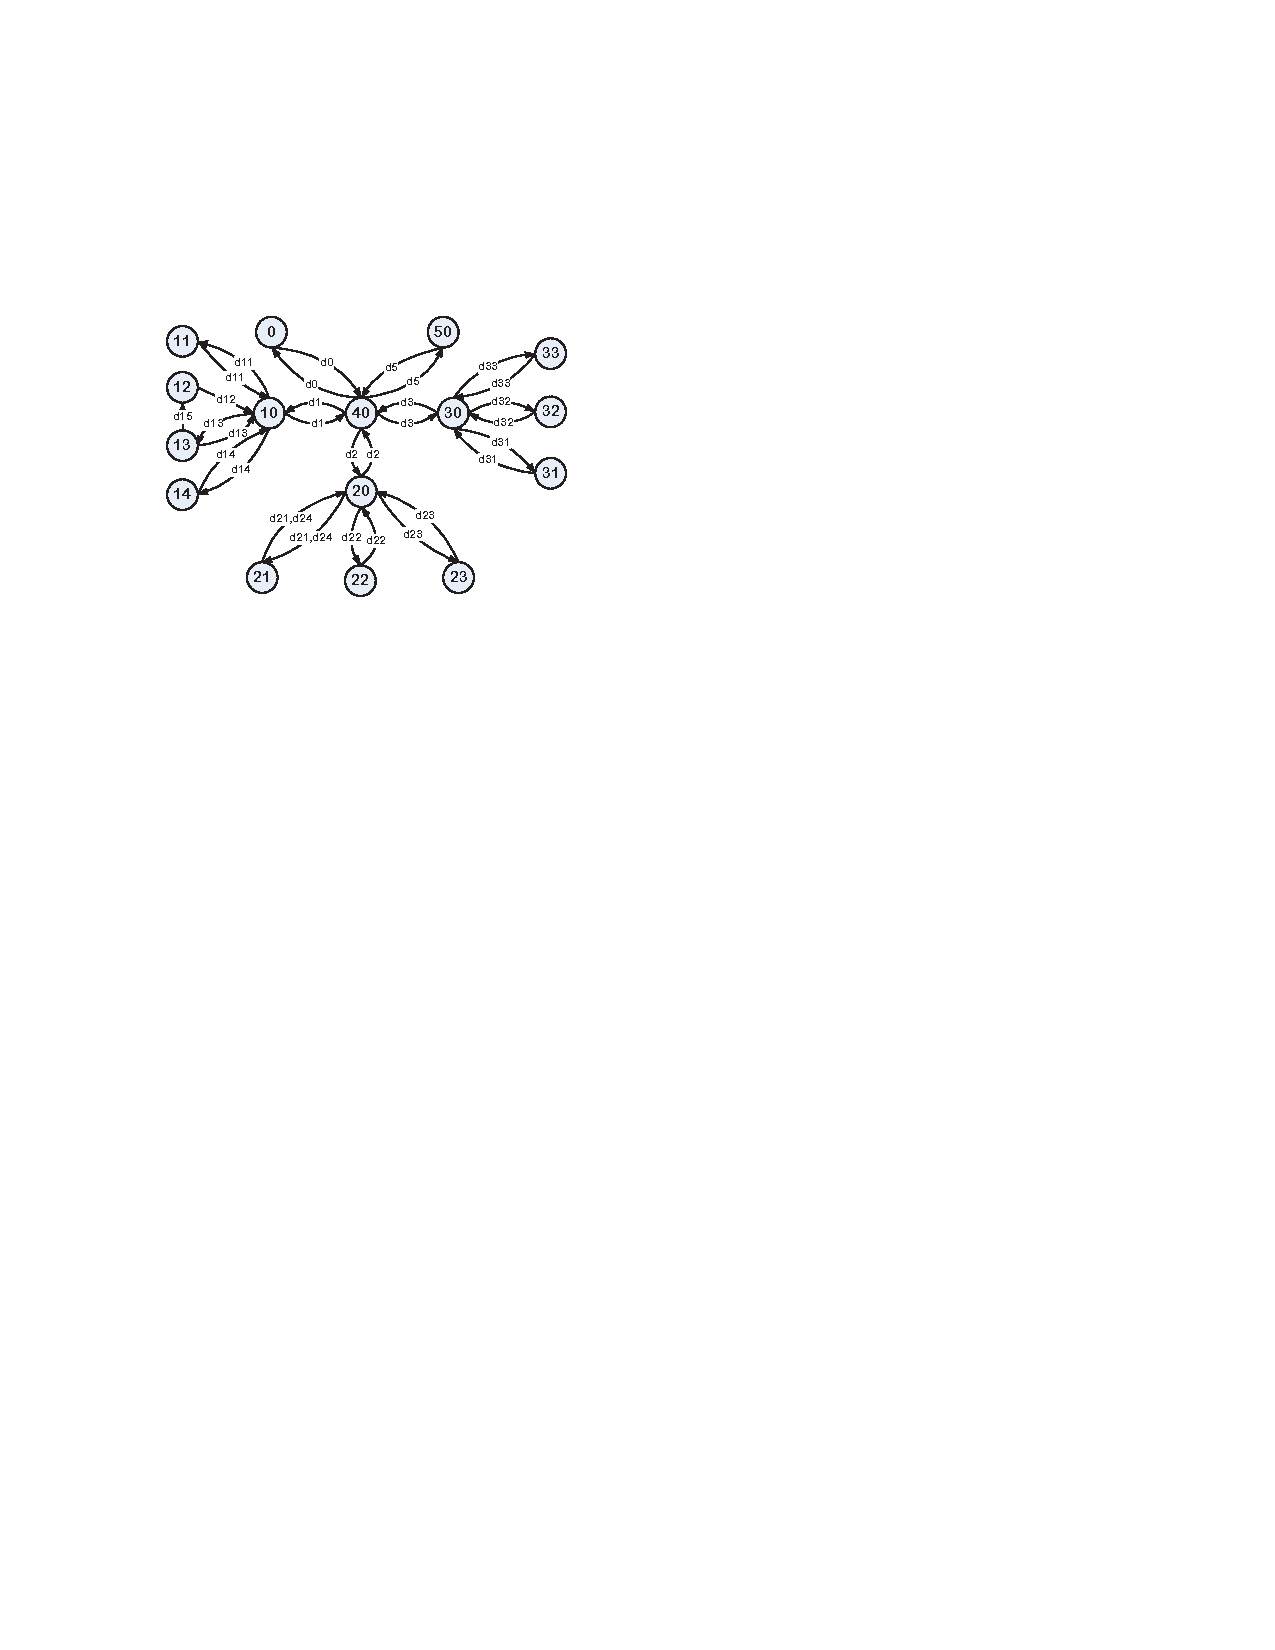
\includegraphics[width=0.8\columnwidth]{figures/2-5/2-5-2.pdf}
  \end{figure}
  \vspace{-10pt}
  \begin{block}{Accessibility Base Graph}
    \textrm{
    \ssize{
    \begin{itemize}
      \item $G_{accs} = \{V, E_a, L\}$
      \item $V = \mathcal{S}_{partition}$ is the set of vertices
      \item $E_a = \{ (v_i, v_j, d_k) | (v_i, v_j) \in D2P(d_k) \}$ is the set of labeled, directed edges
      \item $L = \mathcal{S}_{door}$ is the set of edge labels
    \end{itemize}
    }
    }
  \end{block}

\end{columns}

\end{frame}

%------------------------------------------------

\begin{frame}
\frametitle{Distance-Aware Model}

\fsize{\textrm{The $G_{accs}$ graph does not capture indoor distance information. \conceptbf{Extended Graph Model} is proposed to integrate indoor distances into the graph in a seamless way. \emph{Minimum Indoor Walking Distance}(MIWD) is used. }}

\begin{block}{Extended Graph Model $G_{dist} = \{ V, E_a, L, f_{dv}, f_{d2d} \}$}
  \textrm{
  \begin{sitemize}
    \item $V = \mathcal{S}_{partition}$ is the set of vertices
    \item $E_a = G_{accs}.E_a$
    \item $L = \mathcal{S}_{door}$ is the set of edge labels
    \item $f_{dv} = \mathcal{S} \times V \rightarrow \mathcal{R} \cup \{ \infty \}$ maps an edge to a distance value.
    \begin{equation*}
      f_{dv} = \left\{\begin{matrix}
                \max_{p \in v_j}|| d_i, p || , & if~~ v_j \in D2P_{\sqsupset};
                \\
                \infty , & otherwise.
                \end{matrix}\right.
    \end{equation*}
    \item $f_{d2d} = V \times \mathcal{S}_{door} \times \mathcal{S}_{door} \rightarrow \mathcal{R} \cup \{ \infty \}$ maps a 3-tuple to a distance value.
    \begin{equation*}
      f_{dv} = \left\{\begin{matrix}
                || d_i, d_j ||_{v_k} , & if~~ d_i \in P2D_{\sqsupset}(v_k) and d_j \in P2D_{\sqsubset}(v_k);
                \\
                \infty , & if~~ d_i = d_j and d_i,d_j \in P2D(v_k);
                \\
                0 , & otherwise.
                \end{matrix}\right.
    \end{equation*}
  \end{sitemize}
  }
\end{block}

\end{frame}

%------------------------------------------------

\begin{frame}
\frametitle{Indoor Distance Computation: \emph{door-to-door distance}}

\begin{columns}[c]

  \column{0.52\textwidth}
  \begin{figure}[tb]
    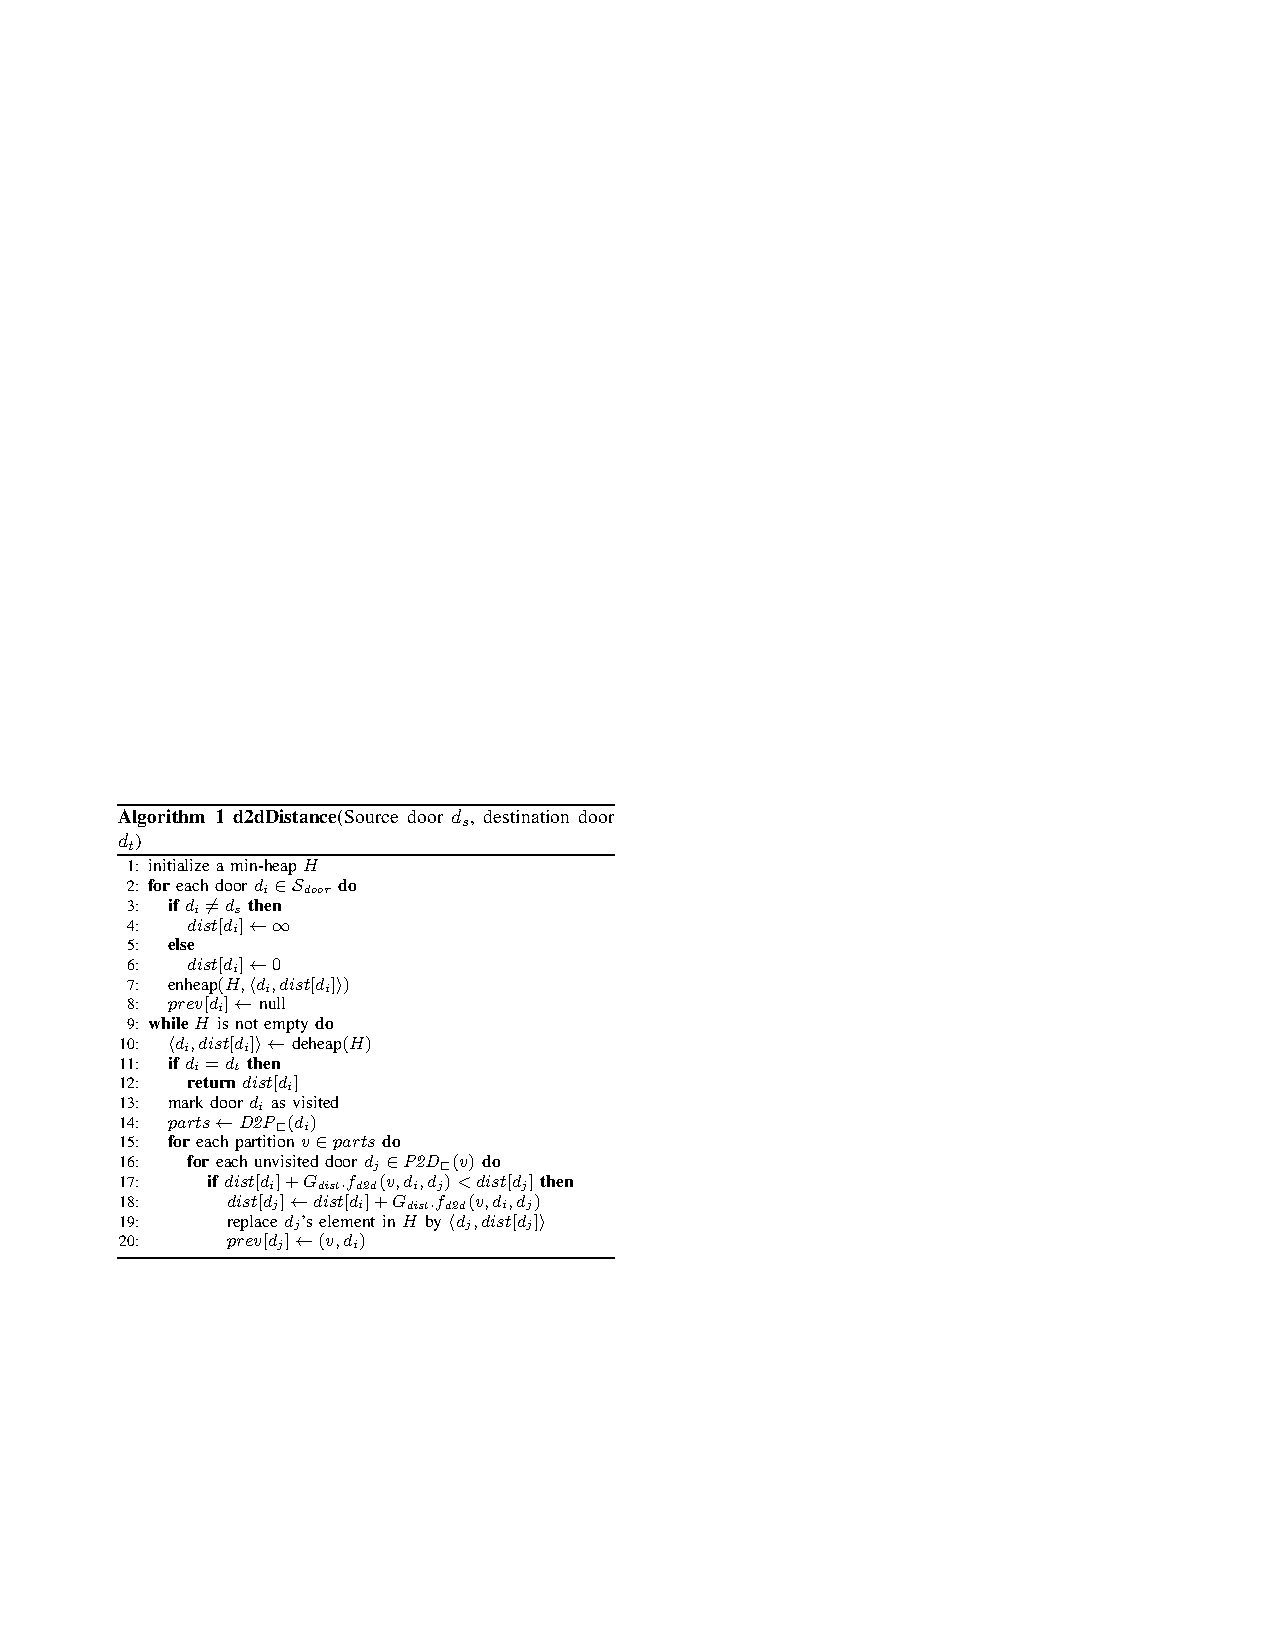
\includegraphics[width=\columnwidth]{figures/2-5/2-5-3.pdf}
  \end{figure}

  \column{0.48\textwidth}


\end{columns}

\end{frame}

%------------------------------------------------

\begin{frame}
\frametitle{Indoor Distance Computation: \emph{point-to-point distance}}

\begin{columns}[c]

  \column{0.52\textwidth}
  \begin{figure}[tb]
    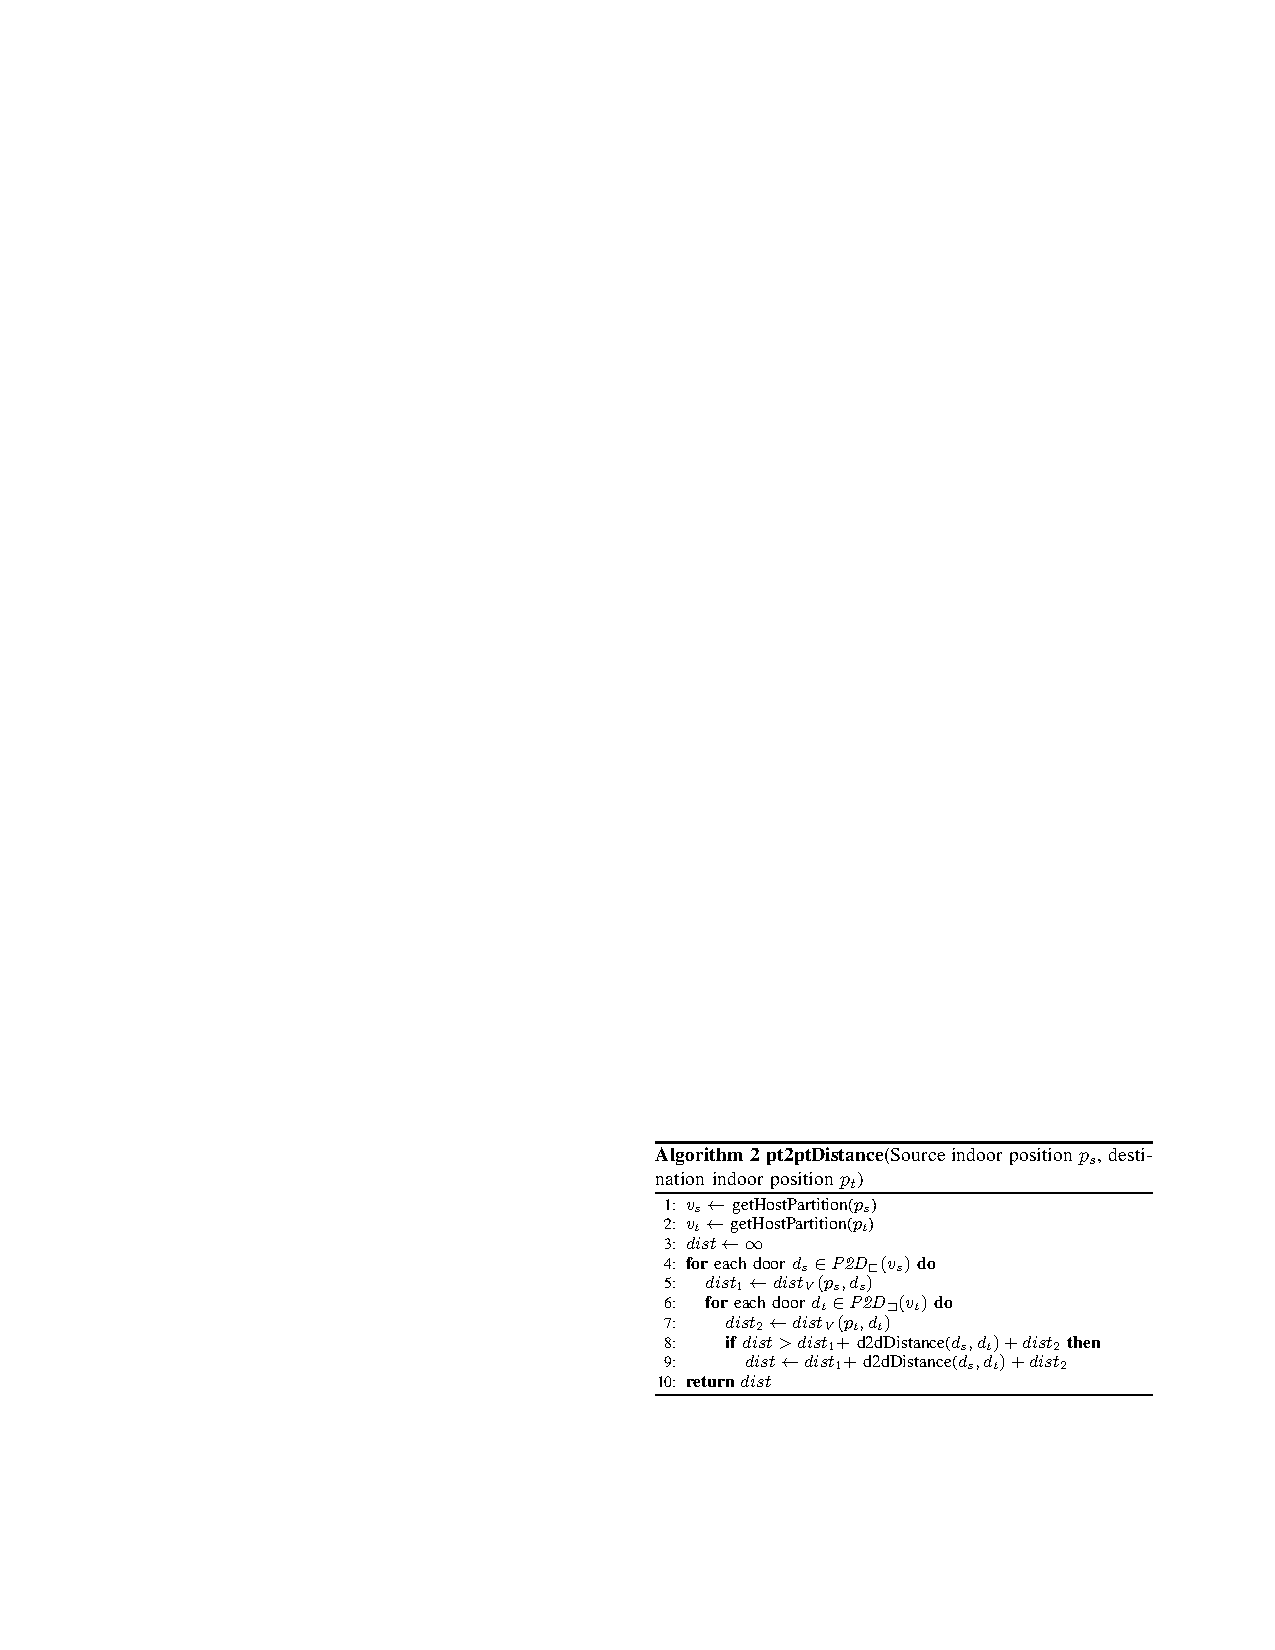
\includegraphics[width=\columnwidth]{figures/2-5/2-5-4.pdf}
  \end{figure}

  \column{0.48\textwidth}


\end{columns}

\end{frame}

%------------------------------------------------

\begin{frame}
\frametitle{Indoor Distance Computation: \emph{point-to-point distance} (I)}

\begin{columns}[c]

  \column{0.52\textwidth}
  \begin{figure}[tb]
    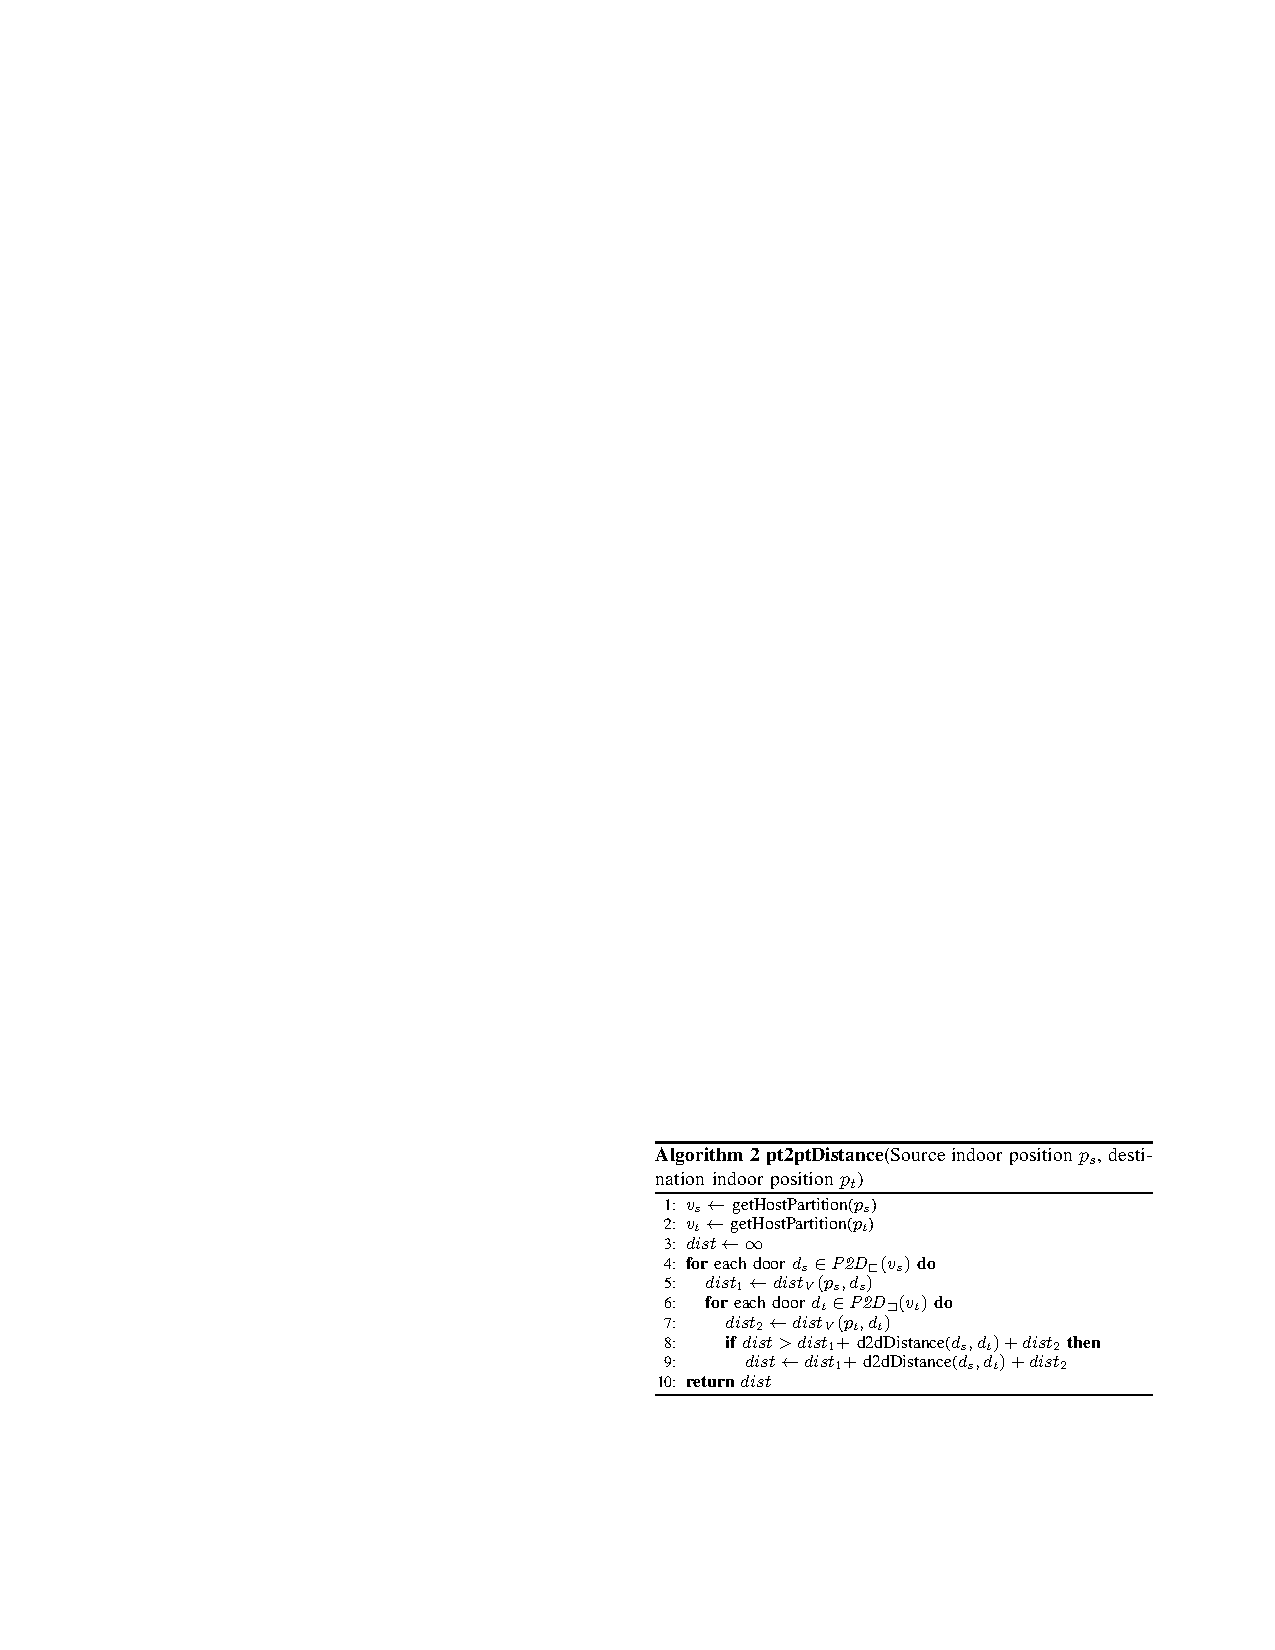
\includegraphics[width=\columnwidth]{figures/2-5/2-5-4.pdf}
  \end{figure}

  \column{0.48\textwidth}


\end{columns}

\end{frame}

%------------------------------------------------

\begin{frame}
\frametitle{Indoor Distance Computation: \emph{point-to-point distance} (II)}

\begin{columns}[c]

  \column{0.4\textwidth}
  \begin{figure}[tb]
    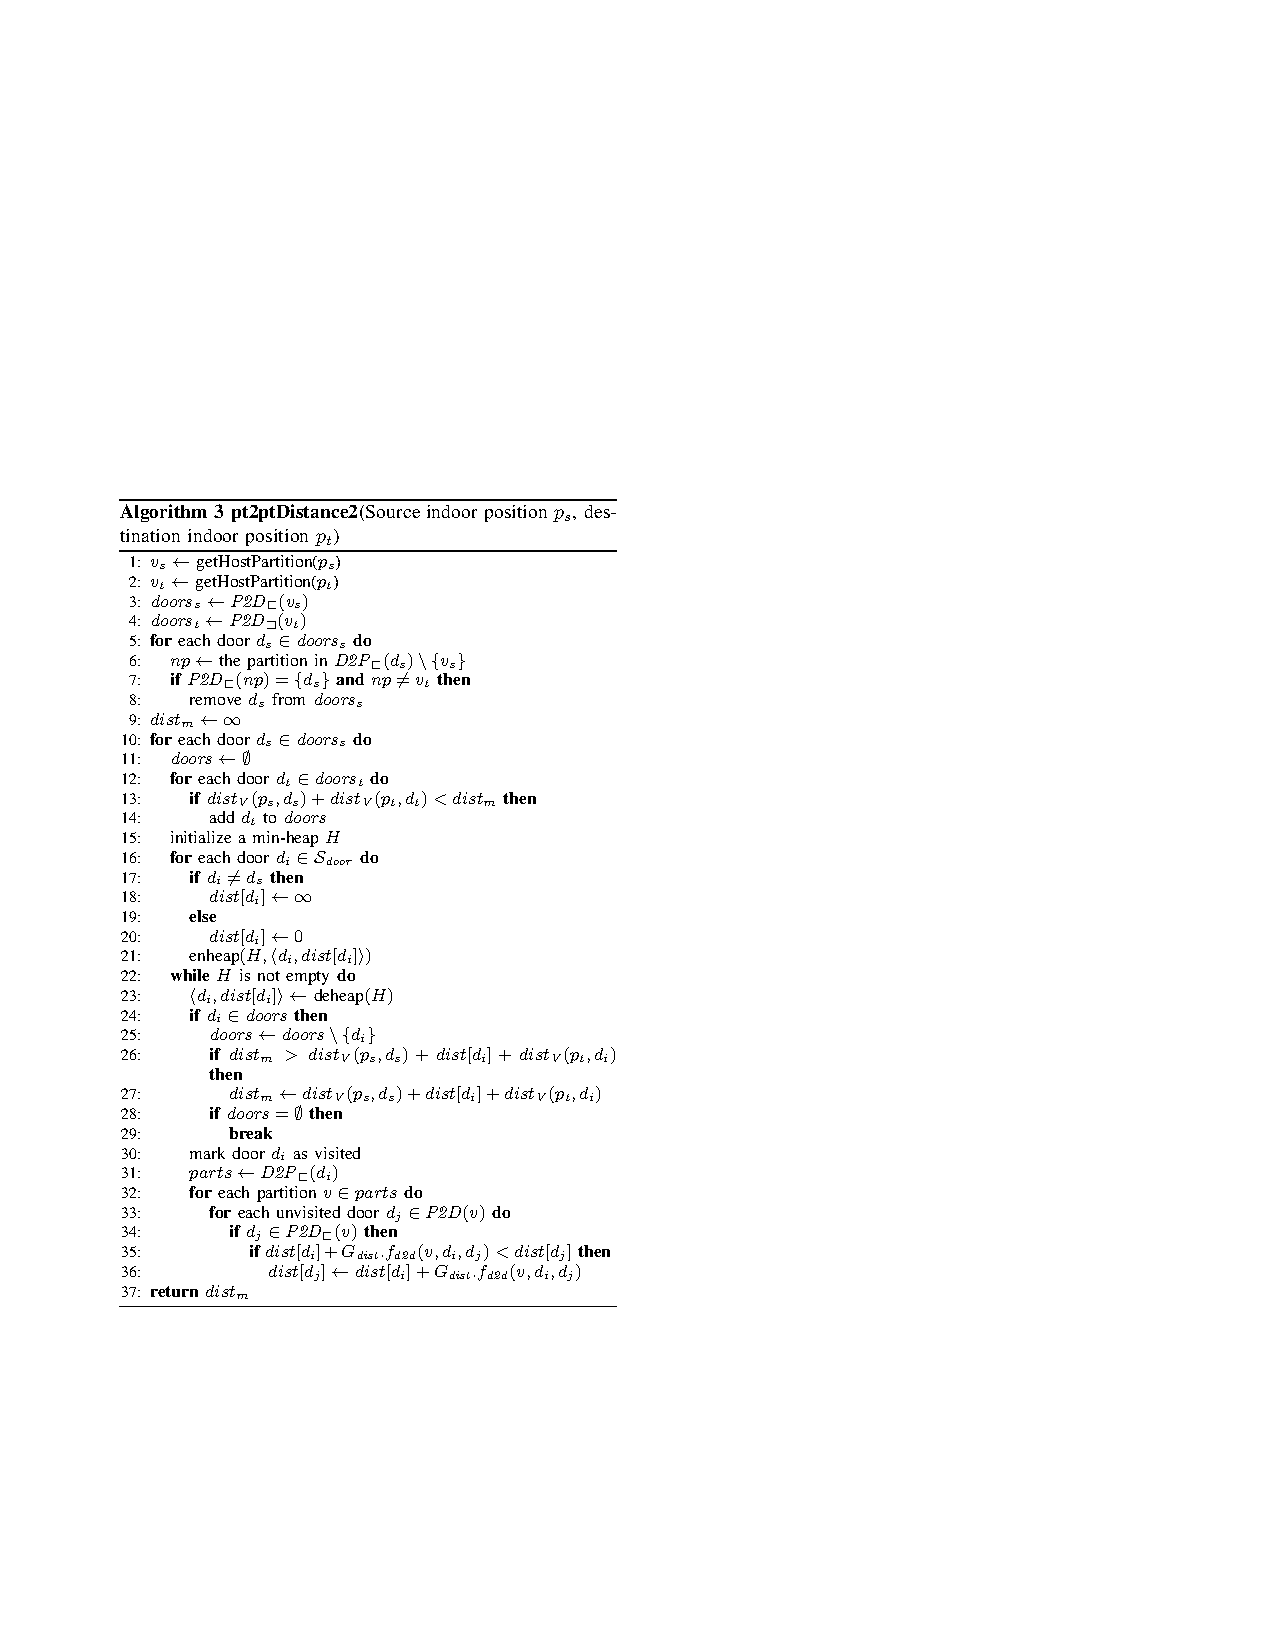
\includegraphics[width=\columnwidth]{figures/2-5/2-5-5.pdf}
  \end{figure}

  \column{0.48\textwidth}


\end{columns}

\end{frame}


% %------------------------------------------------
%
% \begin{frame}
% \frametitle{Indoor Distance Computation: \emph{point-to-point distance} (III)}
%
% \begin{columns}[c]
%
%   \column{0.52\textwidth}
%   \begin{figure}[tb]
%     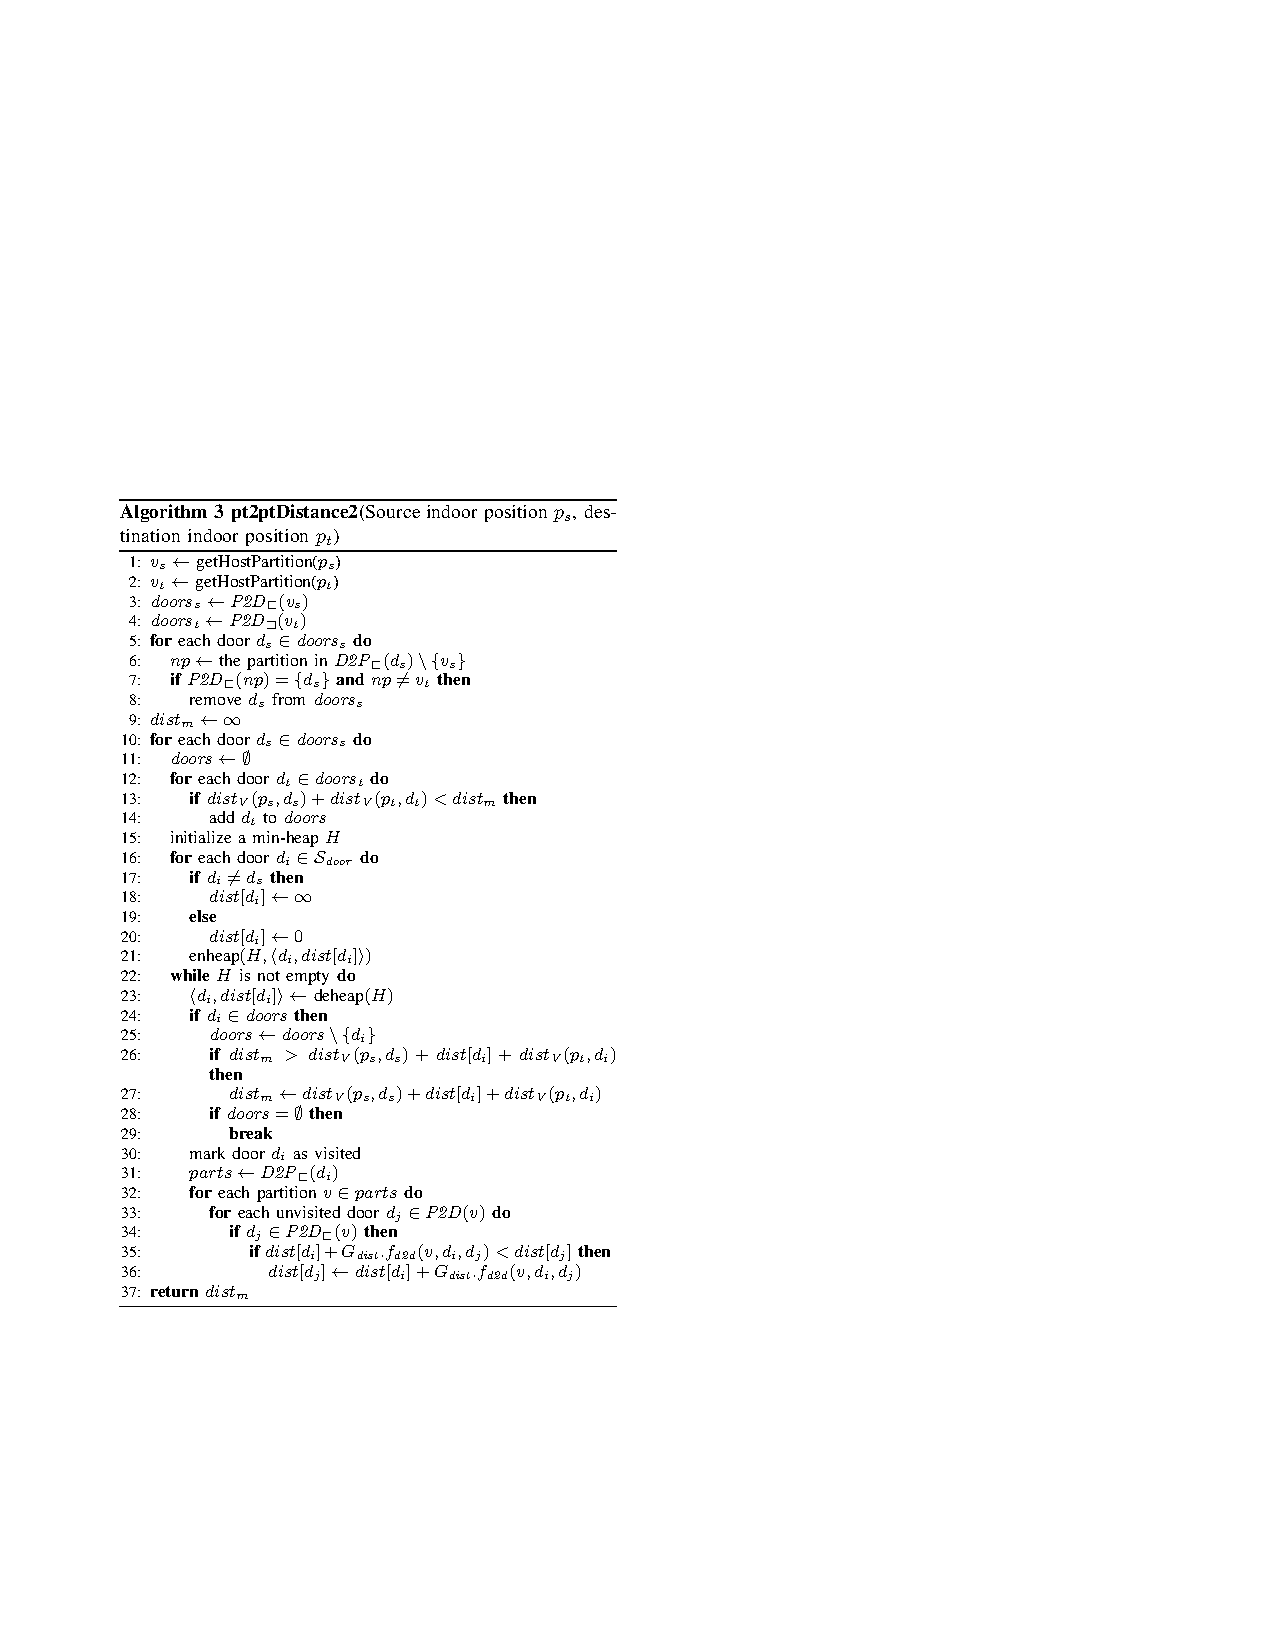
\includegraphics[width=\columnwidth]{figures/2-5/2-5-5.pdf}
%   \end{figure}
%
%   \column{0.48\textwidth}
%
%
% \end{columns}
%
% \end{frame}
